\section {Oszillatoren}
\subsection {Definition und Klassifikation von Oszillatoren \normalfont{\small{(Skript S.6-2)}}} 
\raggedright

Oszillatoren werden in zwei Hauptgruppen unterteilt:
\begin{compactitem}
    \item \textbf{Abgestimmte} Oszillatoren aus einem Verstärker und einem Frequenz bestimmenden Newtzwerk, die in \textbf{positiver} Rückkopplung betrieben werden.
    \item \textbf{Nichtabgestimmte} oder schaltende Oszillatoren bestehen dagegen aus einem Schaltelement mit mindestens zwei stabilen Zuständen (\textbf{Multivibrator}) und einem Integrator oder Tiefpassfilter, welches zwischen den Zuständen des Schaltelementes umgeladen wird. Die Umladezeit des Integrators ist hier Frequenz bestimmend während die Amplitude üblicherweise durch die Pegel des Schaltelementes gegeben ist.
\end{compactitem}
 
\centering
\begin{figure}[h!]
  \centering
  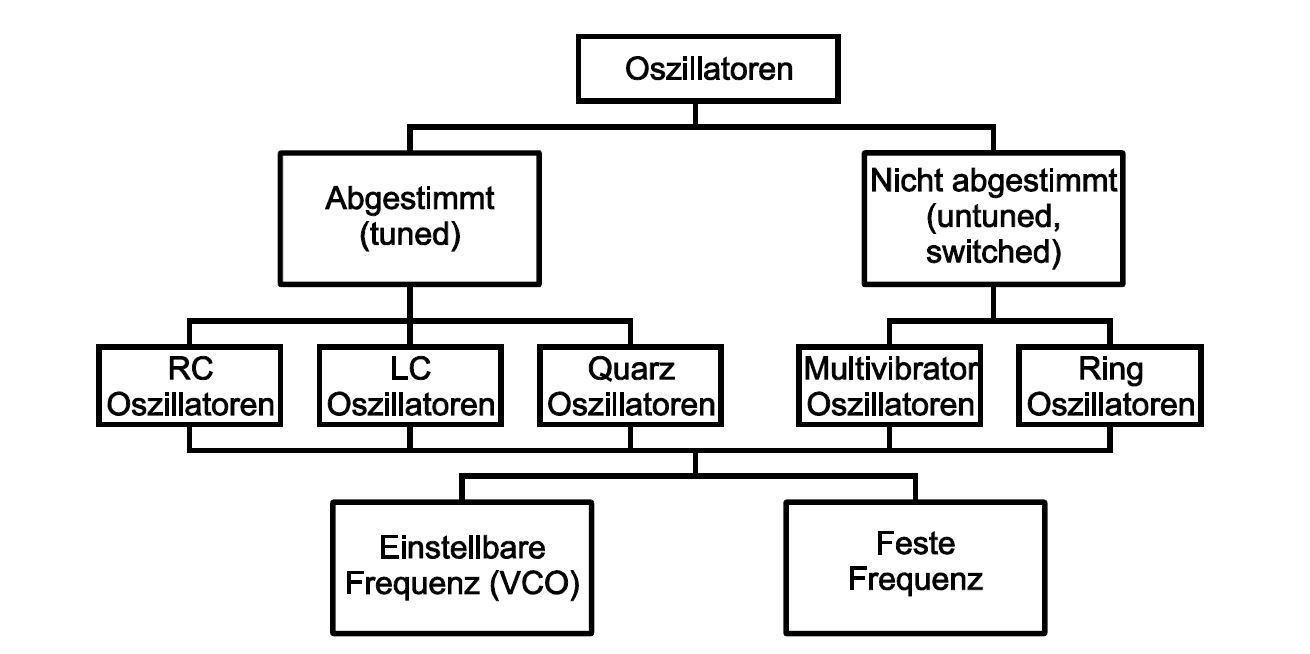
\includegraphics[width=0.8\textwidth]{images/Klassifikation_Oszillatortypen}
  \subcaption*{Klassifikation von Oszillatortypen}
\end{figure}

\FloatBarrier
\subsection{Oszillatorgrundprinzipien \normalfont{\small{(Skript S.6-4)}}}
\subsubsection{Die Rückkopplungsschleife (Feedback Loop) bei abgestimmten Oszillatoren}
\begin{figure}[h!]
	% minipage mit (Blind-)Text
	\begin{minipage}{0.3\textwidth} 
	  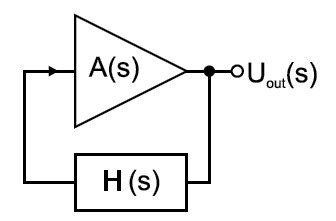
\includegraphics[width=1.0\textwidth]{images/Blockdiagramm_Oszillator}
	 % \subcaption*{Blockdiagramm eines Oszillators}
	% \label{Text}
	\end{minipage}
	\begin{minipage}{0.4\textwidth}
	  \begin{equation*}
        \text{\textbullet }A_cl(s) =\frac{A_(s)}{1-A(s) \cdot H(s)} = \frac{A(s)}{1-T(s)}
      \end{equation*}
      \begin{compactitem}
        \item Schwingbedingung: $T(s)=1$\\
        \item Anschwingbedingung: $T(s)>1$\\ 
      \end{compactitem}
	\end{minipage}
\end{figure}
\raggedright

\FloatBarrier
\subsubsection{Amplitudenstabilisierung}
Die Schleifenverstärkung ist eine Funktion der Signalamplitude (nichtlinearer Effekt). Für anwachsenden Amplitude wird die Verstärkung kleiner. 
\begin{figure}[h!]
	% minipage mit (Blind-)Text
	\begin{minipage}{0.4\textwidth} 
	  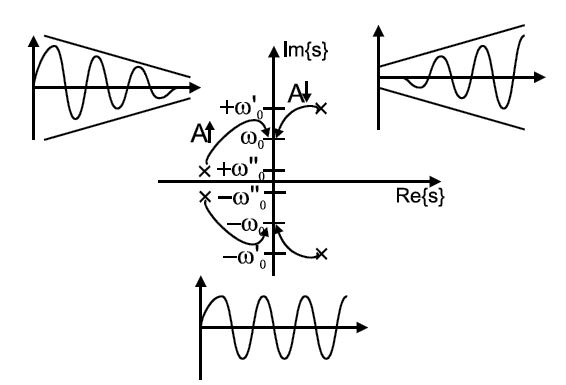
\includegraphics[width=1\textwidth]{images/Pollage_Regelung}
	 % \subcaption*{Regelung der Pollage durch amplitudenabhängige Vertärkung}
	\end{minipage}
	\begin{minipage}{0.5\textwidth}
      \begin{compactenum}
        \item Anfangszustand: $T(s)=1$ (Pol befindet sich in rechter s-Halbene)
        \item Signalamplitude steigt exponentiell an.
        \item dadurch wird $T(s)$ reduziert
        \item dadurch werden Pole nach imag.-Achse verschoben (grenzstabil)
        \item falls Pol in inke s-Halbebene gelangt, geschiet das umgekehrte
        \item dadurch werden Pole auf Achse gehalten
      \end{compactenum}
	\end{minipage}
\end{figure}

\FloatBarrier
\subsection{Abgestimmte Oszillatoren \normalfont{\small{(Skript S.6-7)}}}

\begin{multicols}{3}
\subsubsection{LC-Oszillatoren}
	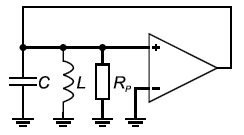
\includegraphics[width=0.3\textwidth]{images/LC-Oszillator}
	%\subcaption*{Regelung der Pollage durch amplitudenabhängige Vertärkung}
	\begin{equation*} 
        \begin{split} 
          \omega_0=\frac{1}{\sqrt{LC}}
        \end{split} 
    \end{equation*}
    \hfill \columnbreak
    
    \subsubsection{Colpitts-Ozsillator}
    \begin{equation*} 
        \begin{split} 
            &T(s) = \frac{-A}{1+sR(C_1+C_2)+s^2LC_2+s^3RLC_1C_2}\\\\
            &\omega _0 = \frac{1}{\sqrt{L\frac{C_1 C_2}{C_1+C_2}}}\\\\
            &A =\frac{C_2}{C_1} \quad \quad \text{beim Anschwingen gilt:} \quad \quad A \geq\frac{C_2}{C_1} \\
            &\text{(A = Amplitude)} \\
        \end{split} 
    \end{equation*}
    
    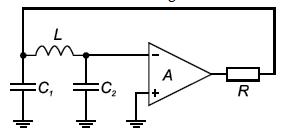
\includegraphics[width=0.3\textwidth]{images/Colpitts-Oszillator}
    \hfill \columnbreak
\end{multicols}

\FloatBarrier
\subsubsection{Quarz-Oszillator \normalfont{\small{(Skript S.6-8)}}}
\vspace{-1.05cm}
\begin{figure}[h!]
	% minipage mit (Blind-)Text
	\begin{minipage}{0.3\textwidth} 
	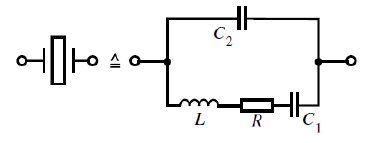
\includegraphics[width=1\textwidth]{images/Ersatzschaltbild_Schwingquarz}
	%\subcaption*{Regelung der Pollage durch amplitudenabhängige Vertärkung}
	\end{minipage}
	\begin{minipage}{0.6\textwidth}
	   Durch anlegen eine Wechselspannung an den Quarz, erhält man eine (bwz. mehrere) Resonsanzfrequenz(en).
       Eigenschaften von Schwingkreisen mit Quarz:
      \begin{compactitem}
        \item sehr temperaturstabil
        \item hohe Güte
        \item hohe Stabilität
        \item Typische Fehlertoleranz ($\frac{\Delta f}{f}$): +/- 20ppm (steigt jedoch quadratisch mit der Abweichung von der optimalen Temperatur (bei Uhrenquarz 25$^\circ$C)) $\rightarrow$ $\quad-0.04ppm/^\circ \text{C}^2$ (typ)\\
        $\frac{\Delta f}{f}=10^{-6}...10^{-10}$
        \item Anschwingbedingung: $g_m \geq R_s\cdot4\omega_0^2C_0 ^2+\frac{4}{R_p}+\frac{1}{R_0}$
        \begin{compactitem}
          \item Es gilt: $ C_0 = C_p+C_1C_2/(C_1+C2)$
        \end{compactitem} 
      \end{compactitem} 
	\end{minipage}
	% minipage mit (Blind-)Text
	\begin{minipage}{0.3\textwidth} 
	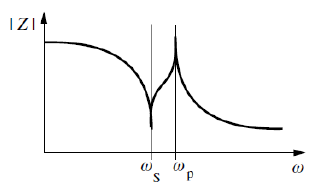
\includegraphics[width=1.0\textwidth]{images/Impedanz(Frequenz)_Schwingquarz}
	%\subcaption*{Regelung der Pollage durch amplitudenabhängige Vertärkung}
	\end{minipage}
	\begin{minipage}{0.6\textwidth}
      %\raggedright
      \vspace{0.5cm}
      Bei der Impedanz eines Schwingquarzes sieht man zwei wesentliche Eigenschaften:
      \begin{compactitem}
        \item zwei Resonanzfrequenzen: Serien- $(Im\{Z(\omega)\}=0)$ und Prallelresonanz $(Im\{Z(\omega)\}=\infty)$
        \item Impedanz ist weitgehend kapazitiv. Induktiv im Bereich:\\ $(\omega_s < \omega < \omega_p)$\\
      \end{compactitem}
      \begin{equation*} 
        \begin{split} 
         & Z (\omega)=\frac{s^2+\omega _s ^2}{sC_p(s^2+\omega_p ^2)} \quad \text{für } Z(s) = jX(\omega): \quad X(\omega)=-\frac{1}{\omega C_p}\cdot \frac{\omega^2-\omega_s ^2}{\omega^2-\omega_p ^2}\\\\
        \end{split} 
      \end{equation*}
	\end{minipage}
\end{figure}

\FloatBarrier
\subsection{Nichtabgestimmte Oszillatoren \normalfont{\small{(Skript S.6-10)}}}
\subsubsection{Multivibrator-Oszillatoren}
\begin{figure}[h!]
	% minipage mit (Blind-)Text
	\begin{minipage}{0.3\textwidth} 
	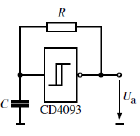
\includegraphics[width=0.8\textwidth]{images/Multivibrator_Komp}
	%\subcaption*{Regelung der Pollage durch amplitudenabhängige Vertärkung}
	\end{minipage}
	\begin{minipage}{0.6\textwidth}
      \begin{compactitem}
        \item max. Komperator Ausgangsspannung:\quad $L_+=V_+$
        \item min. Komperator Ausgnagsspannung:\quad $L_-=V_-$
        \item Teilungsfaktor: $\beta$\\\\
       \end{compactitem}
      \begin{equation*} 
        \begin{split} 
          &f_{osc}=\frac{1}{T} \quad \text{mit} \quad T=\tau \cdot ln \frac{(\beta L_- - L_+)(\beta L_+ - L_-)}{(\beta L_+ - L_+)(\beta L_- - L_-)}\\\\
          & \text{für} \quad   L_+=L_-: \quad  T=2\tau \cdotln\frac{\beta+1}{\beta-1}\\\\
        \end{split} 
      \end{equation*}
	\end{minipage}
\end{figure}

\begin{multicols}{2}
\subsubsection*{LM555}
	    \begin{tabular}{Llll}
           & Ladezeit:             & $t_1=0.693\cdot(R_A+R_B)C$    \\
           & Entladezeit:          & $t_2=0.693\cdot R_B \cdot C$   \\
           &  Frequenz:             & $f=\frac{1}{T}=\frac{1.44}{(R_A+2\cdot R_B)C}$    \\
    \end{tabular}
    \hfill \columnbreak
    
    \subsubsection*{Ringoszillator}
	\begin{equation*} 
        \begin{split} 
          f_{osc} =\frac{1}{2n\cdot t_g} \quad \quad \Delta\varphi =\frac{180^\circ}{2n}   \\\\
        \end{split} 
      \end{equation*}
\end{multicols}

\FloatBarrier
\subsection{Spannungsgesteuerte Oszillatoren (VCO) \normalfont{\small{(Skript S.6-17)}}}
Elemente für Realisierung eines VCO's (Siehe Beispiele ab S.6-20 Skript):

\begin{compactitem}
   \item \textbf{FET im Anlaufgebiet}: Arbeitet als gesteuerter Widersand
   \item \textbf{Binär geschaltete Elemente}
   \item \textbf{Diode im Sperrbereich}: Steuerbarer Kondensator $C_D(V_{SP})=\frac{C_0}{(1+\frac{V_{SP}}{\Phi})^m}$
   \item \textbf{Referenzspannung beim Multivibrator (LM555)}: Variieren der Auf- und Entladezeiten
   \item \textbf{Delay-Interpolation}: $f_{min} =\frac{1}{2n_{max}\cdot t_g} \quad \text{und} \quad f_{max} =\frac{1}{2n_{min}\cdot t_g}$
\end{compactitem}


